\PassOptionsToPackage{table}{xcolor}

\documentclass[oneside]{ausarbeitung}

\bibliography{references}

\usepackage{tikz}
\usepackage{listings}
\lstset{numbers=left, numberstyle=\tiny, numbersep=5pt}
\lstset{language=C}
\lstset{ % ... whatever was already there ...
        literate=% ... any other literates already there ...
                 {!}{!}1
                 {?}{?}1
                 {:}{:}1
}

\usepackage{dirtree}

\usepackage{xcolor}

\definecolor{lightblue}{RGB}{117, 200, 255}
\definecolor{lightgreen}{RGB}{84, 255, 129}

\colorlet{punct}{red!60!black}
\definecolor{background}{HTML}{EEEEEE}
\definecolor{delim}{RGB}{20,105,176}
\colorlet{numb}{magenta!60!black}

\lstdefinelanguage{json}{
    basicstyle=\normalfont\ttfamily,
    numbers=left,
    numberstyle=\scriptsize,
    stepnumber=1,
    numbersep=8pt,
    showstringspaces=false,
    breaklines=true,
    literate=
     *{0}{{{\color{numb}0}}}{1}
      {1}{{{\color{numb}1}}}{1}
      {2}{{{\color{numb}2}}}{1}
      {3}{{{\color{numb}3}}}{1}
      {4}{{{\color{numb}4}}}{1}
      {5}{{{\color{numb}5}}}{1}
      {6}{{{\color{numb}6}}}{1}
      {7}{{{\color{numb}7}}}{1}
      {8}{{{\color{numb}8}}}{1}
      {9}{{{\color{numb}9}}}{1}
      {:}{{{\color{punct}{:}}}}{1}
      {,}{{{\color{punct}{,}}}}{1}
      {\{}{{{\color{delim}{\{}}}}{1}
      {\}}{{{\color{delim}{\}}}}}{1}
      {[}{{{\color{delim}{[}}}}{1}
      {]}{{{\color{delim}{]}}}}{1},
}

% syntax definition for glsl
%
% author: Sebastian Schäfer
% contact: 23@numb3r23.net

\lstdefinelanguage{GLSL}
{
	sensitive=true,
	alsoletter={\#},
	morekeywords=[1]{
		attribute, const, uniform, varying,
		layout, centroid, flat, smooth,
		noperspective, break, continue, do,
		for, while, switch, case, default, if,
		else, in, out, inout, float, int, void,
		bool, true, false, invariant, discard,
		return, mat2, mat3, mat4, mat2x2, mat2x3,
		mat2x4, mat3x2, mat3x3, mat3x4, mat4x2,
		mat4x3, mat4x4, vec2, vec3, vec4, ivec2,
		ivec3, ivec4, bvec2, bvec3, bvec4, uint,
		uvec2, uvec3, uvec4, lowp, mediump, highp,
		precision, sampler1D, sampler2D, sampler3D,
		samplerCube, sampler1DShadow,
		sampler2DShadow, samplerCubeShadow,
		sampler1DArray, sampler2DArray,
		sampler1DArrayShadow, sampler2DArrayShadow,
		isampler1D, isampler2D, isampler3D,
		isamplerCube, isampler1DArray,
		isampler2DArray, usampler1D, usampler2D,
		usampler3D, usamplerCube, usampler1DArray,
		usampler2DArray, sampler2DRect,
		sampler2DRectShadow, isampler2DRect,
		usampler2DRect, samplerBuffer,
		isamplerBuffer, usamplerBuffer, sampler2DMS,
		isampler2DMS, usampler2DMS,
		sampler2DMSArray, isampler2DMSArray,
		usampler2DMSArray, struct
	},
	morekeywords=[2]{
		radians,degrees,sin,cos,tan,asin,acos,atan,
		atan,sinh,cosh,tanh,asinh,acosh,atanh,pow,
		exp,log,exp2,log2,sqrt,inversesqrt,abs,sign,
		floor,trunc,round,roundEven,ceil,fract,mod,modf,
		min,max,clamp,mix,step,smoothstep,isnan,isinf,
		floatBitsToInt,floatBitsToUint,intBitsToFloat,
		uintBitsToFloat,length,distance,dot,cross,
		normalize,faceforward,reflect,refract,
		matrixCompMult,outerProduct,transpose,
		determinant,inverse,lessThan,lessThanEqual,
		greaterThan,greaterThanEqual,equal,notEqual,
		any,all,not,textureSize,texture,textureProj,
		textureLod,textureOffset,texelFetch,
		texelFetchOffset,textureProjOffset,
		textureLodOffset,textureProjLod,
		textureProjLodOffset,textureGrad,
		textureGradOffset,textureProjGrad,
		textureProjGradOffset,texture1D,texture1DProj,
		texture1DProjLod,texture2D,texture2DProj,
		texture2DLod,texture2DProjLod,texture3D,
		texture3DProj,texture3DLod,texture3DProjLod,
		textureCube,textureCubeLod,shadow1D,shadow2D,
		shadow1DProj,shadow2DProj,shadow1DLod,
		shadow2DLod,shadow1DProjLod,shadow2DProjLod,
		dFdx,dFdy,fwidth,noise1,noise2,noise3,noise4,
		EmitVertex,EndPrimitive
	},
	morekeywords=[3]{
		gl_VertexID,gl_InstanceID,gl_Position,
		gl_PointSize,gl_ClipDistance,gl_PerVertex,
		gl_Layer,gl_ClipVertex,gl_FragCoord,
		gl_FrontFacing,gl_ClipDistance,gl_FragColor,
		gl_FragData,gl_MaxDrawBuffers,gl_FragDepth,
		gl_PointCoord,gl_PrimitiveID,
		gl_MaxVertexAttribs,gl_MaxVertexUniformComponents,
		gl_MaxVaryingFloats,gl_MaxVaryingComponents,
		gl_MaxVertexOutputComponents,
		gl_MaxGeometryInputComponents,
		gl_MaxGeometryOutputComponents,
		gl_MaxFragmentInputComponents,
		gl_MaxVertexTextureImageUnits,
		gl_MaxCombinedTextureImageUnits,
		gl_MaxTextureImageUnits,
		gl_MaxFragmentUniformComponents,
		gl_MaxDrawBuffers,gl_MaxClipDistances,
		gl_MaxGeometryTextureImageUnits,
		gl_MaxGeometryOutputVertices,
		gl_MaxGeometryOutputVertices,
		gl_MaxGeometryTotalOutputComponents,
		gl_MaxGeometryUniformComponents,
		gl_MaxGeometryVaryingComponents,gl_DepthRange,
		\#version,core
	},
	morecomment=[l]{//},
	morecomment=[s]{/*}{*/},
	%morecomment=[l][keywordstyle4]{\#},
}


\newcommand*{\captionsource}[2]{%
  \caption[{#1}]{%
    #1%
    \\\hspace{\linewidth}%
    \textbf{Quelle:} #2%
  }%
}

\newcommand*{\quotize}[1]{\glqq #1\grqq}
\hypersetup{colorlinks=false,allcolors=black}

% ----------------------------------------------------------------------

\begin{document}

\selectlanguage{ngerman}

%--- Art der Arbeit
% Erlaubte Werte:
% Praxissemesterbericht, Projektbericht, Bachelorarbeit oder                                % Masterarbeit
\doctype{Bachelorarbeit}

%--- Studiengang:
\depname{Medieninformatik}

\title{WebGPU}

\author{Laurin Agostini}
\matrikelnr{60526}

\examinerA{Prof.~Dr.~Winfried~Bantel}
\examinerB{Prof.~Dr.~Carsten~Lecon}
\date{XX. Juni 2020}

%--- Titelseite Anzeigen
\maketitle
\cleardoublepage

%---
\pagenumbering{roman}
\setcounter{page}{1}


%--- Eidesstattliche Erklärung anzeigen
\makeaffirmation
\cleardoublepage

%---
\chapter*{Kurzfassung}
\addcontentsline{toc}{chapter}{Kurzfassung}
In dieser Bachelorarbeit geht es um die neuartige Grafik-API WebGPU, die einen Nachfolger zu WebGL darstellt. Mit WebGPU ist es möglich, detaillierte 3D-Szenen, aufwendige Simulationen und XXX in Echtzeit direkt im Webbrowser zu berechnen und darzustellen. 

%-----------------------------------------------------------------------
\cleardoublepage
\addcontentsline{toc}{chapter}{Inhaltsverzeichnis}
\tableofcontents

%---
\addcontentsline{toc}{chapter}{Abbildungsverzeichnis}
\listoffigures

%---
\addcontentsline{toc}{chapter}{Tabellenverzeichnis}
\listoftables

\addcontentsline{toc}{chapter}{Listings}
\lstlistoflistings

%---
\chapter*{Abkürzungsverzeichnis}
\addcontentsline{toc}{chapter}{Abkürzungsverzeichnis}
\begin{acronym}[JSON]  % Längstes Kürzel in der nachfolgenden
                       % Liste um die Breite der Spalte für die
                       % Abkürzungen zu bestimmen.

%% Eintrag: \acro{Referenzname}[Kürzel]{Langform}
%% Im Text wird die Abkürzung dann mit \ac{Referenzname} benutzt.
\acro{json}[JSON]{JavaScript Object Notation}
\acro{CPU}[CPU]{Central Processing Unit (dt. Hauptprozessor)}
\acro{GPU}[GPU]{Graphics Processing Unit (dt. Grafikprozessor)}
\acro{SMT}[SMT]{Simultaneous Multithreading}
\acro{PCIe}[PCIe]{Peripheral Component Interconnect Express}
\acro{API}[API]{Application Programming Interface (dt. Programmierschnittstelle)}
\acro{WSL}[WSL]{Windows Subsystem for Linux}
\acro{GLSL}[GLSL]{OpenGL Shading Language}
\end{acronym}
%---
\cleardoublepage
\pagenumbering{arabic}
\setcounter{page}{1}

% ----------------------------------------------------------------------
\chapter{Einleitung}
\label{cha:einleitung}

\section{Motivation}
\label{sec:motivation}

\section{Problemstellung und -abgrenzung}
\label{sec:problemstellung}

\section{Ziel der Arbeit}
\label{sec:ziel}

\section{Vorgehen}
\label{sec:vorgehen}


% ---
\chapter{Grundlagen}
\label{cha:grundlagen}

\section{GPU}
\label{sec:GPU}

\subsection{Aufgaben und Unterschied zur CPU}
\label{sub:GPU_tasks}
Wie der Name, \textit{\textbf{Grafik}prozessor} oder \textit{\textbf{graphics} processing unit}, schon andeutet, ist der Primärzweck einer \ac{GPU} die Erstellung und Manipulation von Bildinhalten und anschließender Ausgabe dieser an ein Anzeigegerät. Während eine \ac{CPU} generell darauf ausgelegt ist, ein weites Spektrum von Aufgaben sequenziell bearbeiten zu können, ist eine \ac{GPU} darauf spezialisiert möglichst viele einfache Aufgaben, insbesondere Fließkommaoperationen, parallel zu bearbeiten. Diesen Unterschied sieht man direkt, wenn man die Leistungsdaten aktueller \ac{CPU}s und \ac{GPU}s vergleicht:

\begin{minipage}{1.0\textwidth}
\begin{center}
\begin{tabular}{ |l|r|r| }
    \hline
    Name & Anzahl Kerne & Basis-/Turbotakt (MHz) \\
    \hline
    \multicolumn{3}{|c|}{High-end} \\
    \hline
    \rowcolor{lightblue}
    Intel® Core™ i9-9900K \cite{intel:i9_9900k} & 8 & 3.600 / 5.000 \\
    \rowcolor{lightgreen}
    NVIDIA GeForce RTX 2080Ti \cite{nvidia:rtx_2080ti} & 4.352 & 1.350 / 1.545 \\
    \hline
    \multicolumn{3}{|c|}{Low-end} \\
    \hline
    \rowcolor{lightblue}
    Intel® Core™ i3-9100 \cite{intel:i3_9100} & 4 & 3.600 / 4.200 \\
    \rowcolor{lightgreen}
    NVIDIA GeForce GTX 1650 \cite{nvidia:gtx_1650} & 896 & 1.485 / 1.665 \\
    \hline
\end{tabular}
\end{center}
Legende: \colorbox{lightblue}{\ac{CPU}} \colorbox{lightgreen}{\ac{GPU}}
\end{minipage}

Hier sieht man sofort, dass \ac{GPU}s eine um mehrere Größenordnungen höhere Anzahl von Kernen haben, welche allerdings mit einer niedrigeren Taktrate laufen. Zwar konnte in den letzten Jahren ein starker Anstieg von Prozessorkernen in Endbenutzer-\ac{CPU}s beobachtet werden, doch auch eine explizite Workstation-\ac{CPU}, wie ein AMD Ryzen™ Threadripper™ 3990X \cite{amd:threadripper_3990x} mit 64 physischen und durch \ac{SMT} 128 logischen Prozessorkernen ist weit von den Kernzahlen einer aktuellen Einstiegs-\ac{GPU} entfernt. Wie schon angemerkt, kann man die Prozessorkerne von \ac{CPU}s und \ac{GPU}s nicht direkt vergleichen, jedoch zeigen sie deutlich die Spezialisierung der \ac{GPU}s auf parallele Verarbeitung mit einem erhöhtem Datendurchsatz. 

Zu den klassischen Aufgaben einer \ac{GPU} gehören Grafik-, Rechen-, Medien- und Displayfunktionalitäten. Durch die fortlaufende Entwicklung von fest in die Hardware programmierte Abläufe zu frei programmierbaren Anwendungen (ähnlich zu einer \ac{CPU}), werden jedoch immer mehr Anwendungen möglich, welche als \textbf{GPUCompute} zusammengefasst werden. Dies führte auch dazu, dass man in den letzten Jahren einen enormen Anstieg von \ac{GPU}s in Rechenzentren zum Beschleunigen von Anwendungen wie zum Beispiel \textit{machine learning} oder \textit{crypto mining}, beobachten konnte. Da sich \hyperref[cha:webgpu]{WebGPU} jedoch eher auf den klassischen Aufgabenbereich der \ac{GPU} bezieht, und dafür eine moderne Schnittstelle bereitstellt, wird sich im folgenden primär auf diese bezogen.

\subsection{Integrierte und dedizierte GPUs}
\label{sub:GPU_dedicated_integrated}
Mittlerweile haben die meisten Endbenutzer-\ac{CPU}s eine integrierte \ac{GPU} (oft auch \textbf{iGPU} genannt) um die üblichen Multimediaaufgaben zu beschleunigen und Last von der \ac{CPU} zu nehmen. Integrierte \ac{GPU}s sind aber für aufwendige Berechnungen wie zum Beispiel für grafikintensive Anwendungen nicht ausreichend. Dafür werden dedizierte Grafikkarten benötigt, welche der \ac{GPU} dedizierten (daher der Name) Arbeitsspeicher und oft auch eine aktive Kühlung bereitstellen. Grafikkarten werden heutzutage meist über \ac{PCIe} angeschlossen.

\begin{figure}
    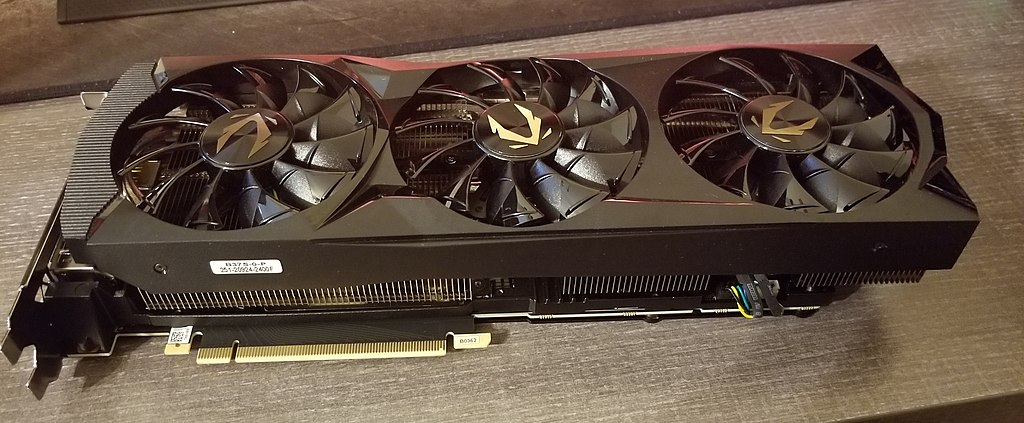
\includegraphics[width=\textwidth]{images/1024px-Zotac_Gaming_GTX_2080_ti.jpg}
    \caption{Beispiel einer Grafikkarte (Zotax Gaming 2080 ti) \cite{2080_ti_graphics_card}}
    \label{fig:2080_ti_graphics_card}
\end{figure}

\subsection{Geschichte \cite[Vgl.][]{gpu_history}}
\label{sub:GPU_history}
\textit{Der Begriff \quotize{\ac{GPU}} wurde erst 1999 von NVIDIA eingeführt, jedoch werden im folgenden der Einfachheit halber alle vorherigen Chips mit ähnlicher Funktion unter dem Begriff \quotize{\ac{GPU}} zusammengefasst.}

Bis in die frühen 1980er Jahre waren \ac{GPU}s nicht mehr als integrierte Bildspeicher und dafür zuständig einfache Linienformen auf den Rasterbildschirm zu zeichnen. Erst ab 1987 wurden weitere Funktionen hinzugefügt. So zum Beispiel Rasterung von Polygonenflächen (anstatt von Polygonkanten), Vertex Beleuchtung, Tiefenpuffer und Farbüberblendung. Im Jahre 1992 wurde von Silicon Graphics Inc. mit OpenGL, die bis heute meist verwendete und unterstützte \ac{API} für Grafikprogrammierung eingeführt.

\section{Rendering-Pipeline}
\label{sec:render_pipeline}
\begin{quote}
The main function of the [graphics rendering] pipeline is to generate, or \textit{render}, a two-dimensional image, given a virtual camera, three-dimensional objects, light sources, and more. The rendering pipeline is thus the underlying tool for real-time rendering.

-- Real-Time Rendering \cite[S. 11]{real_time_rendering}
\end{quote}


\subsection{Architektur}
Grundsätzlich besteht die Rendering-Pipeline aus vier Abschnitten, die mehr oder weniger frei programmierbar sind (siehe Abbildung \ref{fig:render_pipeline}). Generell läuft der Abschnitt \textit{Anwendung} auf der \ac{CPU} (kann aber auch mithilfe von \ac{GPU}-Compute auf der \ac{GPU} implementiert werden) und beschreibt die Logik der Anwendung. Die drei folgenden Abschnitte \textit{Geometrieverarbeitung}, \textit{Rasterung} und \textit{Pixelverarbeitung} laufen alle auf der \ac{GPU}, wobei die \textit{Geometrie-} und \textit{Pixelverarbeitung} hier frei mit \textit{Shadern} programmierbar sind und die \textit{Rasterung} nur über Parameter konfiguriert werden kann.

\begin{figure}
    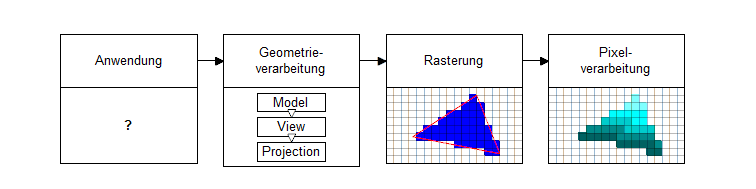
\includegraphics[width=\textwidth]{images/render_pipeline.png}
    \caption{Grundsätzlicher Aufbau der Rendering-Pipeline, unterteilt in die vier Abschnitte \textit{Anwendung}, \textit{Geometrieverarbeitung}, \textit{Rasterung} und \textit{Pixelverarbeitung}}
    \label{fig:render_pipeline}
\end{figure}

\subsection{Anwendung}
Der Abschnitt \textit{Anwendung} kann nicht konkret beschrieben werden, da er sich, wie der Name schon sagt, von Anwendung zu Anwendung unterscheidet. Jedoch kann man grundsätzlich sagen, dass hier die Logik der Anwendung stattfindet, wie zum Beispiel:
\begin{itemize}
\item{Benutzereingaben verarbeiten und auswerten}
\item{Physikberechnungen zwischen den Objekten}
\item{Ressourcen von der Festplatte laden}
\end{itemize}
Damit bereitet der Abschnitt \textit{Anwendung} die Daten für die restlichen Abschnitte vor und entscheidet, was dafür in Betrachtung gezogen wird (zum Beispiel nur Objekte in Blickrichtung der virtuellen Kamera).

\subsection{Geometrieverarbeitung}
Die \textit{Geometrieverarbeitung} ist dafür zuständig, die Geometriedaten (\textit{vertices} (Eckpunkte)) für die Rasterung vorzubereiten. Dafür müssen die \textit{vertices} meist zuerst von ihrer lokalen Position (innerhalb des Objektes) in die Position innerhalb des Sichtfeldes der virtuellen Kamera umgewandelt werden. 

\begin{figure}
    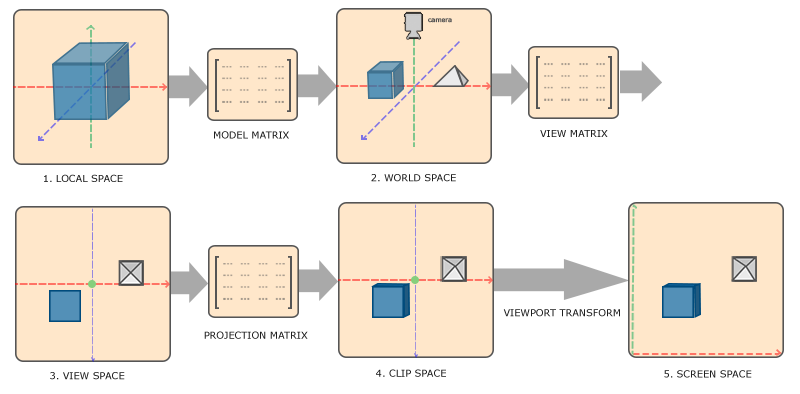
\includegraphics[width=\textwidth]{images/mvp_matrix.png}
    \caption{Transformation von Objekt bezogenen Vertexdaten in den \textit{world space}, dann in den \textit{view space} und schlussendlich in den \textit{clip space}. Die finale Umwandlung vom \textit{clip space} in den \textit{screen space} passiert dabei automatisch und verschiebt den Ursprung von der Mitte in entweder die ober oder untere (abhängig von der verwendeten Grafik-API) linke Ecke.}
    \label{fig:mvp_matrix}
\end{figure}

Dies passiert normalerweise mithilfe mehrerer Matrizen (siehe Abbildung \ref{fig:mvp_matrix}). Dabei wandelt die \textit{Model}-Matrix die lokalen Vertexdaten in das globale (\textit{world}) Koordinatensystem um. Die \textit{View}-Matrix wandelt dann die transformierten Daten wiederum in das lokale System der virtuellen Kamera um. Schlussendlich projiziert die \textit{Projection}-Matrix die Vertexdaten aus dem dreidimensionalen Raum auf die Bildebene. 

Die \textit{Model}-Matrix ist dabei abhängig von der Transformation des jeweiligen Objektes im \textit{world space}. Aus der Transformation der Kamera ergibt sich die \textit{View}-Matrix und die \textit{Projection}-Matrix wird aus den speziellen Eigenschaften der Kamera (Sichtfeld und \textit{near-}/\textit{far-plane} bei einer perspektivischen Projektion) gebildet. Manchmal werden die einzelnen Matrizen \textit{Model}, \textit{View} und \textit{Projection} auch zur sogenannten \textit{ModelViewProjection}-Matrix zusammengefasst um die Anzahl der Vektor-Matrix-Multiplikationen zu verringern.

Der Abschnitt Geometrieverarbeitung ist bis auf die finale Umwandlung vom \textit{clip space} in den \textit{screen space} frei programmierbar. Dabei wird ein sogenannter \textit{Shader} (Programm, das auf der \ac{GPU} läuft, kommt vom englischen \textit{to shade} (dt. schattieren), also dem Bestimmen der Helligkeitswerte eines Pixels) für jeden Vertex aufgerufen. Da dieser Abschnitt aber auf der \ac{GPU} läuft, kann man die Geometrieverarbeitung aber nicht mit einer üblichen Programmiersprache für \ac{CPU}s implementieren, sondern muss eine Programmiersprache für \textit{Shader}, wie zum Beispiel GLSL verwenden. Die Syntax von \ac{GLSL} ist dabei stark an der von C angelehnt. 

In Listing \ref{lst:vertex_shader} sieht man die Implementierung der Geometrieverarbeitung in der, bei dieser Arbeit entstandenen, \textbf{spider}-Engine. Dabei werden die Matrizen \textit{Model}, \textit{View} und \textit{Projection} einzeln dem Shader übergeben und sind für alle Shader-Ausführungen (für dieses Objekt) konstant. Jedoch unterscheiden sich bei jeder Ausführung die Daten des jeweiligen Vertex, für den der Shader ausgeführt wird. Diese spezifischen Daten bekommt der Shader in den 4 Eingangsparametern ab Zeile 14 übergeben:
\begin{itemize}
\item{\textit{inPosition}: die Position des Vertex innerhalb des Objektes}
\item{\textit{inTexCoords}: die Texturkoordinaten des Vertex, zur späteren Bestimmung von Materialeigenschaften in der Pixelverarbeitung}
\item{\textit{inNormal}: die Normale des Vertex, meist aus den Normalen der angrenzenden Polygonflächen berechnet}
\item{\textit{inTangent}: die Tangente des Vertex, wird zur Anwendung von \textit{normal maps} in der Pixelverarbeitung benötigt}
\end{itemize}

Die 4 Ausgangsparameter ab Zeile 19 werden dann später, nach der Interpolation bei der Rasterung, in der Pixelverarbeitung benutzt. Wobei der Prefix \textit{frag} hier für \textit{fragment} steht, was eine alternative Bezeichnung für einen Pixel ist.
\begin{itemize}
\item{\textit{fragPosWorld}: die Position des Pixels im \textit{world space}}
\item{\textit{fragTexCoords}: die Texturkoordinaten des Pixels}
\item{\textit{fragNormal}: die Normale des Pixels}
\item{\textit{fragTangent}: die Tangente des Pixels}
\end{itemize}

\textit{gl\_Position} ist ein von \ac{GLSL} reservierter Ausgansparameter in dem die berechnete Vertexposition, zur weiteren Nutzung in folgenden Pipeline-Abschnitten, im \textit{clip space} gespeichert werden soll. Die lokale Vertexposition wird dabei zuerst vom lokalen System des Objektes mithilfe der \textit{Model}-Matrix in den \textit{world space} transformiert.  Diese Position wird dann einerseits direkt in \textit{fragPosWorld} abgespeichert und anderseits mithilfe der \textit{View}- und \textit{Projection}-Matrizen in den \textit{clip space} transformiert und in \textit{gl\_Position} gespeichert. Der Wert für \textit{fragTexCoords} wird direkt von \textit{inTexCoords} übernommen, da er unabhängig vom jeweiligen Koordinatensystem ist. Da \textit{inNormal} und \textit{inTangent} jeweils normalisierte Vektoren (also Richtungen) darstellen, können diese nicht mit der normalen \textit{Model}-Matrix in den \textit{world space} transformiert werden. Dazu muss erst die Transponierte der inversen \textit{Model}-Matrix gebildet werden. Mit dieser können dann \textit{fragNormal} und \textit{fragTangent} jeweils von \textit{inNormal} und \textit{inTangent} berechnet werden.

\begin{minipage}{\textwidth}
\begin{lstlisting}[language=GLSL, label={lst:vertex_shader}, caption={Beispiel eines Vertex Shaders in \ac{GLSL}, welcher so in der \textbf{spider}-Engine verwendet wird}]
#version 450
#extension GL_ARB_separate_shader_objects : enable

layout(set = 0, binding = 0) uniform Model {
    mat4 model;
};

layout(set = 0, binding = 1) uniform Camera {
    mat4 view;
    mat4 proj;
    vec3 pos;
} cam;

layout(location = 0) in vec3 inPosition;
layout(location = 1) in vec2 inTexCoords;
layout(location = 2) in vec3 inNormal;
layout(location = 3) in vec3 inTangent;

layout(location = 0) out vec3 fragPosWorld;
layout(location = 1) out vec2 fragTexCoords;
layout(location = 2) out vec3 fragNormal;
layout(location = 3) out vec3 fragTangent;

void main() {
    vec3 pos_world = vec3(model * vec4(inPosition, 1.0));
    gl_Position = cam.proj * cam.view * vec4(pos_world, 1.0);
    fragPosWorld = pos_world;
    fragTexCoords = inTexCoords;
    mat3 to_world = mat3(transpose(inverse(model)));
    fragNormal = to_world * inNormal;
    fragTangent = to_world * inTangent;
}
\end{lstlisting}
\end{minipage}
\subsection{Rasterung}

\subsection{Pixelverarbeitung}


\section{Grafik-API}
\subsection{Die Anfänge}
\subsection{•}
\subsection{\quotize{Moderne} Grafik-APIs}

\chapter{WebGPU}
\label{cha:webgpu}

\section{GPU im Web}
Mit dem rasanten Beliebtheitszuwachs von webbasierten Anwendungen, die nicht lokal installiert werden müssen und direkt im Webbrowser benutzt werden können, wurden auch Rufe nach einer Möglichkeit, 3D-Grafiken effizient in einem Webbrowser anzuzeigen, laut. Mit den beiden im Jahr 2011 eingeführten Web-Grafik-APIs \textit{Stage3D} \cite{adobe:stage3d} als Teil des \textit{Adobe Flash Player} und das offene und nativ in \textit{JavaScript} verfügbare \textit{WebGL} \cite{khronos:webgl} der \textit{Khronos Group}.
\section{Unterschied zu WebGL}
\section{Beschreibung}
\section{Der aktuelle Stand}
\subsection{Spezifikation}
Die Spezifikation \cite{webgpu:api_spec} der \textbf{WebGPU}-\ac{API} ist zum Zeitpunkt des Verfassens dieses Abschnittes (09.06.2020) noch nicht abgeschlossen und wurde auch während dem Verlauf der Arbeit mehrmals erweitert und angepasst.

\subsection{Implementierung}
\textit{Der aktuelle Stand der Implementierung in Webbrowsern kann unter \cite{webgpu:implementation_status} eingesehen werden.}

\subsubsection{Chromium \cite{chromium} / Dawn \cite{google:dawn}}
\textit{Dawn} ist eine Open-Source \textbf{WebGPU}-Implementierung, die in dem Open-Source Webbrowser Chromium verwendet wird. Unter anderem basieren die bekannten Webbrowser \textit{Google Chrome}, \textit{Opera} und seit neustem auch \textit{Microsoft Edge} auf Chromium. 

Die \quotize{native} Implementierung von \textit{Dawn} benutzt dafür die Grafik-APIs der jeweils ausführenden Plattform:

\begin{itemize}
\item{\textit{D3D12} auf Windows 10}
\item{\textit{Metal} auf macOS und iOS}
\item{\textit{Vulkan} auf Windows, Linux und Google eigenen Betriebssystemen (ChromeOS, Android, Fuchsia)}
\item{\textit{OpenGL} wo verfügbar}
\end{itemize}

Das heißt, dass die \textbf{WebGPU}-Befehle hier im Hintergrund die jeweiligen Befehle der nativen Grafik-API aufrufen. Dies hat den Vorteil, dass \textbf{WebGPU} so keinen eigenen Treiber braucht, um mit der \ac{GPU} zu kommunizieren. Da die generelle \textbf{WebGPU}-API-Struktur auch ähnlich zu der Struktur der nativen APIs (bis auf OpenGL) ist, bedeutet dies auch keinen großen Mehraufwand bei der Implementierung und kann sogar teilweise von Codegeneratoren bewerkstelligt werden.

\subsubsection{Firefox Nightly \cite{mozilla:firefox_nightly} / wgpu \cite{mozilla:wgpu}}
\textit{wgpu} ist ebenfalls eine Open-Source \textbf{WebGPU}-Implementierung in der Programmiersprache \textit{Rust}. \textit{wgpu} wird hierbei unter anderem im \textit{Mozilla Firefox}-Webbrowser verwendet und von der \textit{Mozilla Foundation} federführend entwickelt.
\section{Nutzen außerhalb von Grafik}

%---
\chapter{Implementierung einer WebGPU-Applikation}
\label{cha:implementierung}
\textit{Für das in diesem Kapitel beschriebene Projekt wurde Windows 10 mit Ubuntu 19.10 per \ac{WSL} \cite{microsoft:wsl} verwendet. Dabei wurden die Quellcodedateien in Windows erstellt und bearbeitet, aber in Ubuntu benutzt (kompilieren, linken usw.). Deshalb beziehen sich im Folgenden alle Angaben zur Installation oder Benutzung von Werkzeugen auf die jeweilige Linux-Version.}

\section{spider}
\label{sec:spider}
\textit{In diesem Abschnitt wird mit \quotize{der Benutzer}, ein Benutzer der \textbf{spider}-Engine verstanden, also eine Person, die mithilfe der Engine eine eigene Applikation entwickelt. \quotize{Der Benutzer} sollte hier als neutrale Form, die die weibliche, sowie die männliche Form beinhaltet, verstanden werden.}
\subsection{Überblick}
\label{sub:overview}
Mit der parallel zu dieser Arbeit entstandenen \textbf{spider}-Engine, lässt sich mit geringem Aufwand eine Webapplikation zur Darstellung von 3D-Szenen in C/C++ erstellen.
Das Grundgerüst dafür ist sehr minimal (siehe Listing \ref{lst:spider_base}).

\begin{minipage}{\textwidth}
\begin{lstlisting}[language=C, label={lst:spider_base}, caption={Grundgerüst einer Applikation mit der \textbf{spider}-Engine}]
#include "spider/spider.h"

// Create the initial state of your scene
void initApplication();
// Update your scene each frame
bool update(float delta_time_s);

int main() {
	const uint32_t surface_width = 1280;
	const uint32_t surface_height = 720;

	// Initialize the spider engine
	spInit(&(SPInit){
		.surface_size = {
			.width = surface_width,
			.height = surface_height
		},
		.update_func = update,
		.camera = {
			.pos = {0.0f, 2.0f, 5.0f},
			.look_at = {0.0f, 0.0f, 0.0f},
			.mode = SPCameraMode_LookAt,
			.fovy = glm_rad(60.0f),
			.aspect = (float)surface_width / (float) surface_height,
			.near = 0.1f,
		},
	});	
	
	initApplication();
	spStart();
	
	return 0;
}

void initApplication() {
	// Here you can create lights (only spotlights for now),
	// create custom meshes and materials 
	// or load them from glTF files (recommended)
}

bool update(float delta_time_s) {
	// Here you can update your created lights, objects and the main camera
	
	// Return false, if you want to quit the application
	return true;
}
\end{lstlisting}
\end{minipage}

Die \textbf{spider}-Engine ist darauf ausgelegt, mit möglichst wenig Code auf Seiten des Benutzers eine 3D-Applikation zu erstellen. So lässt sich in rund 150 Zeilen Code eine interaktive 3D-Szene mit einem UserInterface (dank integriertem Dear ImGui \cite{dear_imgui}) erstellen (siehe Abbildung \ref{fig:spider_example_sponza} und Anhang \ref{appendix:a}). Trotzdem ist die Funktionalität der \textbf{spider}-Engine sehr beschränkt, wenn man etwas anderes als das Darstellen von 3D-Modellen und eines einfachen UserInterfaces will. Jedoch ist der Verfasser überzeugt, dass es für einfache Prototypen ausreichend ist.

\begin{figure}
    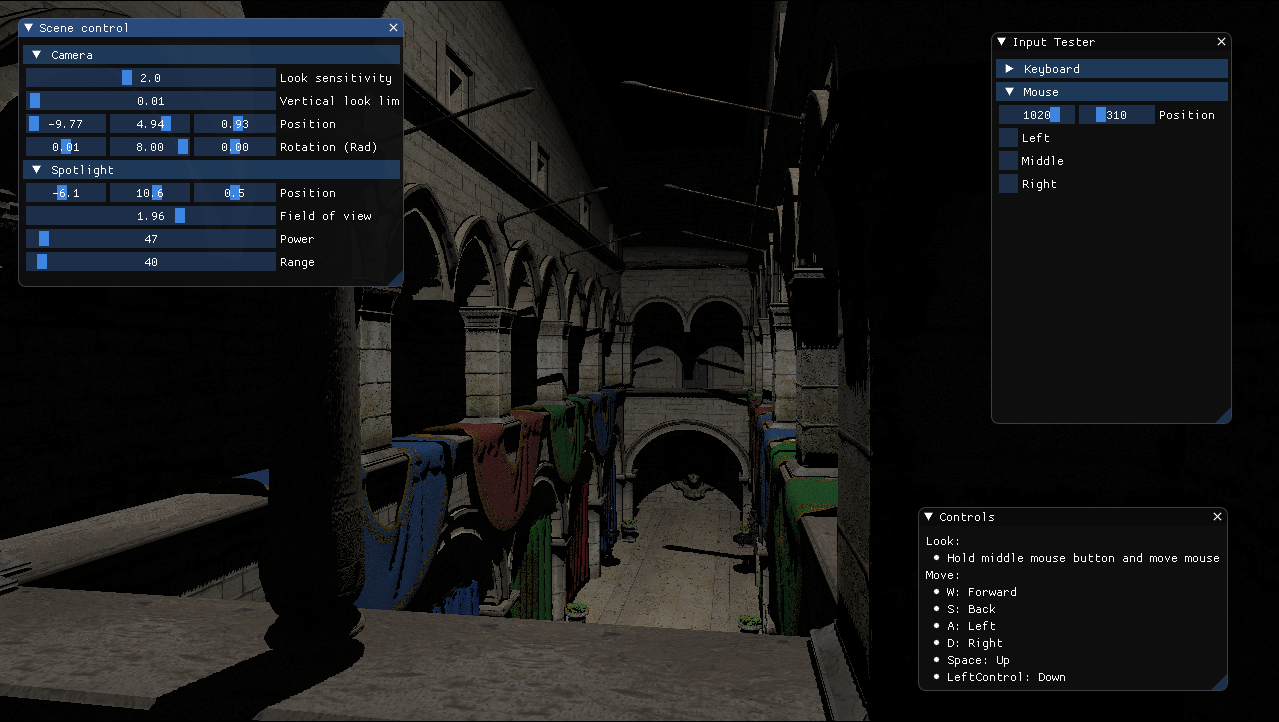
\includegraphics[width=\textwidth]{images/state_of_work_20200608.png}
    \caption{Interaktive 3D-Szene mit UserInterface. Bildschirmaufnahme durch Verfasser.}
    \label{fig:spider_example_sponza}
\end{figure}

\subsection{Codestyle}
\label{sub:codestyle}
\textit{Für das Projekt wurde der C Standard C99 und der von \textbf{Emscripten} verwendete Compiler clang benutzt. Folgende Punkte sollten in allen größeren C-Compilern, die C99 unterstützen, problemlos funktionieren, wurden dort aber nicht getestet.}

Um einen einheitlichen Codestyle zu erhalten, hat der Verfasser sich auf folgende Punkte festgelegt:

\subsubsection{\textit{stdint.h} und \textit{stdbool.h}}
Im Projekt wurden die seit C99 verfügbaren Headerdateien \texttt{stdint.h} und \texttt{stdbool.h} benutzt, um einerseits mehr Kontrolle über den Speicherbedarf der jeweiligen Komponenten zu erlangen und anderseits mehr Kontext zu geben. So ist zum Beispiel bei einer Variable des Typen \texttt{uint8\_t} schnell klar, dass der Verfasser für die Benutzung der Variable nur einen relativ kleinen Bereich an positiven Ganzzahlen beabsichtigt hat. Auch der Typ \texttt{bool} ist im Vergleich zu einem \texttt{int} eindeutig im Bezug auf die Absicht des Verfassers. Interessanterweise wurde beim gesamten Projekt (außer bei der Kommunikation mit den verwendeten Bibliotheken) nur Ganzzahldatentypen ohne Vorzeichen benutzt (\texttt{uint8\_t}, \texttt{uint16\_t}, \texttt{uint32\_t} und \texttt{uint64\_t}).

\subsubsection{Prefixe}
Da es in C keine Namensbereiche, wie zum Beispiel in C++, gibt, werden alle Strukturen, Enums, Funktionen, Preprozessordirektiven und globale Variablen mit einem Prefix versehen (siehe Tabelle \ref{tab:prefixes}). Die Unterscheidung zwischen \textit{öffentlich} und \textit{privat} ist hierbei keine Unterscheidung auf Compilerlevel, sondern nur für den Benutzer, damit dieser erkennen kann, welche Funktionen und Strukturen benutzt werden sollten und welche nur intern genutzt werden.

\begin{table}
\begin{center}
\begin{tabular}{ |l|l|l| }
\hline
\textbf{Typ} & \textbf{Prefix} & \textbf{Beispiel} \\
\hline
\multicolumn{3}{|c|}{\quotize{öffentlich}} \\
\hline
Struktur & \texttt{SP} & \texttt{SPMesh} \\
\hline
Enum & \texttt{SP} & \texttt{SPKey} \\
\hline
Funktion & \texttt{sp} & \texttt{spInit} \\
\hline
Preprozessordirektive & \texttt{SP\_} & \texttt{SP\_INVALID\_ID} \\
\hline
globale Variable & \texttt{sp\_} & \textit{kein Beispiel} \\
\hline
\multicolumn{3}{|c|}{\quotize{privat}} \\
\hline
Struktur & \texttt{\_SP} & \texttt{\_SPRenderPipeline} \\
\hline
Enum & \texttt{\_SP} & \textit{kein Beispiel} \\
\hline
Funktion & \texttt{\_sp} & \texttt{\_spSetupPools} \\
\hline
Preprozessordirektive & \texttt{\_SP\_} & \texttt{\_SP\_MATERIAL\_POOL\_DEFAULT} \\
\hline
globale Variable & \texttt{\_sp\_} & \texttt{\_sp\_state} \\
\hline
\end{tabular}
\end{center}
\caption{Verwendete Prefixe}
\label{tab:prefixes}
\end{table}

\subsubsection{Definition von Strukturen}
Strukturen werden im Projekt wie in Listing \ref{lst:structs} definiert.

\begin{minipage}{\textwidth}
\begin{lstlisting}[language=C, label={lst:structs}, caption={Definition von Strukturen}]
typedef struct MyStructure {
	uint32_t x;
	struct {
		float width;
		float height;
	} size;
} MyStructure;
\end{lstlisting}
\end{minipage}

Dies hat den Vorteil, dass die so definierten Strukturen nicht immer ein vorhergehendes \texttt{struct} bei der Verwendung im Code benötigen. Zusätzlich wird direkt nach dem \texttt{struct} auch der Name der Struktur benötigt, damit diese weiterhin vorwärts deklariert werden kann \cite[vgl.][]{weissflog:structs}. 

Semantisch zusammengehörige Attribute innerhalb einer Struktur werden entweder in eine extra Struktur ausgelagert, oder als anonyme Struktur (siehe \texttt{size} im Beispiel) innerhalb der Struktur definiert. Dadurch kann über \texttt{my\_structure.size.width} auf das Attribut zugegriffen werden.

\subsubsection{\textit{Desc}-Argument}
In vielen Programmiersprachen ist es möglich, beim Aufrufen einer Funktion nur einen Teil der Argumente anzugeben, während die restlichen Argumente mit Standardwerten initialisiert werden. C unterstützt zwar keine Standardargumente, dafür aber ab C99 \textit{Bestimmte Initialisierer (engl. designated initializers)}, was bedeutet, dass man die Felder von Strukturen (und Arrays) mit ihrem jeweiligen Namen (oder Index) in beliebiger Reihenfolge innerhalb einer Initialisierungsanweisung angeben kann. Wenn mindestens ein Feld initialisiert wird, werden alle nicht initialisierten Felder mit \textbf{0} initialisiert. (Zur Verdeutlichung siehe Listing \ref{lst:designated_initializers}). 

\begin{minipage}{\textwidth}
\begin{lstlisting}[language=C, label={lst:designated_initializers}, caption={Beispiele zu bestimmten Initialisierern (Unter Verwendung der in Listing \ref{lst:structs} definierten Struktur \textit{MyStructure})}]
// No guarantee on initialization values
MyStructure my_structure;

// Initialization in field order 
// -> (x = 5, size.width = 3.0f, size.height = 4.0f)
MyStructure my_structure_order = {5, {3.0f, 4.0f}};
MyStructure my_structure_order2 = {5, 3.0f, 4.0f};

// Initialization in field order, rest is zero initialized
// -> (x = 5, size.width = 0.0f, size.height = 0.0f)
MyStructure my_structure_order_zero = {5};

// Initialization with field names
// -> (x = 5, size.width = 3.0f, size.height = 4.0f)
MyStructure my_structure_named = {.size.width = 3.0f, .x = 5, .size.height = 4.0f};
MyStructure my_structure_named2 = {.size = {.width = 3.0f, .height = 4.0f }, .x = 5};

// Initialization with field names, rest is zero initialized
// -> (x = 0, size.width = 3.0f, size.height = 0.0f)
MyStructure my_structure_named_zero = {.size.width = 3.0f};
MyStructure my_structure_named_zero2 = {.size = {.width = 3.0f}};

// Initialization of array fields
// -> (0, 3, 0, 0, 1)
uint32_t array[5] = {
	[1] = 3,
	[4] = 1
};
\end{lstlisting}
\end{minipage}

Im Projekt wird das bei Funktionen mit einer nicht trivialen Argumentliste verwendet. Dabei wird für die jeweilige Funktion eine Struktur mit dem Postfix \texttt{Desc} (für engl. \textit{descriptor}, analog zu den \textbf{WebGPU}-\textit{Descriptor}-Strukturen) definiert. Diese enthält alle benötigten Argumente (mit möglichst sinnvollem Standardwert \textbf{0}). Da es außerdem in C99 möglich ist, einen Zeiger auf ein temporäres Objekt zu erzeugen, hat die jeweilige Funktion nun als einziges Argument einen Zeiger auf ein konstantes Objekt der \texttt{Desc}-Struktur: \texttt{void myFunction(const MyFunctionDesc* desc);}. Nun kann die \texttt{Desc}-Struktur entweder vor dem Aufrufen der Funktion erschaffen und befüllt werden, oder direkt beim Funktionsaufruf initialisiert werden (siehe Listing \ref{lst:function_desc}).

\begin{minipage}{\textwidth}
\begin{lstlisting}[language=C, label={lst:function_desc}, caption={Verwendung einer \textit{Desc}-Struktur zum Übergeben von Argumenten an eine Funktion}]
typedef struct MyFunctionDesc {
	uint32_t values[5];
	const char* name;
} MyFunctionDesc;

void myFunction(const MyFunctionDesc* desc);

MyFunctionDesc my_desc;
my_desc.values[2] = 5;
my_desc.name = "Abc";
myFunction(&my_desc);

myFunction(&(MyFunctionDesc){
	.values = {
		[2] = 5,
	},
	.name = "Abc",
});
\end{lstlisting}
\end{minipage}

\subsubsection{\textit{handles} \cite[Vgl.][]{weissflog:handles}}
\label{subsub:handles}

Die \textbf{spider}-Engine hat das Grundprinzip, dass der Benutzer sich weder um die (De-)Allokation von Speicher, noch über die Referenzierungen zwischen Objekten, kümmern muss und somit den vollen Fokus auf die Erstellung der jeweiligen Applikation richten kann. Dabei soll auch die Speicherverwaltung von erschaffenen Objekten (zum Beispiel ein \texttt{SPMesh}) einzig der \textbf{spider}-Engine überlassen werden. Dabei soll die Engine auch die Möglichkeit haben, die jeweiligen Objekte intern zu verschieben und zu sortieren (bisher nicht benutzt) um den internen Zugriff zu optimieren. Daher kann die Engine nicht direkt einen Zeiger auf ein erschaffenes Objekt liefern, da dieser bei einer Änderung der internen Struktur ungültig wird.

Dafür gibt es für jede \textit{öffentliche} Struktur eine \textit{handle}-Struktur mit Postfix \textit{ID} (zum Beispiel für \texttt{SPMesh} -> \texttt{SPMeshID}) welche eine interne ID (\textit{uint32\_t id}) beinhaltet. Bisher wird die interne ID des \textit{handle} einfach direkt als Index in das interne Array zur Verwaltung der jeweiligen Objekte benutzt, jedoch könnte man hier noch ähnlich zu \cite{weissflog:handles} die unbenutzten Bits (bei zum Beispiel maximal $2^{16} = 65536$ gleichzeitig existierenden Objekten bleiben hier 16 von 32 Bits übrig) zur Versionierung des \textit{handle} verwenden. Um das referenzierte Objekt dann im Anwendungscode zu benutzen kann ein temporärer Zeiger erzeugt werden (siehe Listing \ref{lst:handle}). Dieser Zeiger sollte vom Benutzter nicht gespeichert werden und nur erzeugt werden, wenn das referenzierte Objekt wirklich verwendet (Attribute lesen oder schreiben) wird. Es gibt keine Garantie, dass der Zeiger im nächsten Update noch auf das gleiche Objekt zeigt, oder überhaupt gültig ist.

\begin{minipage}{\textwidth}
\begin{lstlisting}[language=C, label={lst:handle}, caption={Verwendung von \textit{handles}}]
typedef struct SPObject {
	float size;
} SPObject;

typedef struct SPObjectID {
	uint32_t id;
} SPObjectID;

// Store the object handle
SPObjectID object_id;

void init() {
	// Create object and store the handle
	object_id = spCreateObject();
}

void update() {
	// Later use the referenced object
	SPObject* object = spGetObject(object_id);
	// If handle is not valid, spGetObject returns a NULL pointer
	if(object) {
		object->size *= 2.0f;
	}
}
\end{lstlisting}
\end{minipage}

\section{emscripten \cite{emscripten}}
Augenscheinlich wurde das Projekt, das diese Arbeit begleitet hat, in C geschrieben. Da die entstandene Applikation jedoch später in einem Webbrowser laufen und dort die \textbf{WebGPU}-\ac{API} benutzen soll, \textbf{<TODO>}. Dazu wird das Werkzeug \textbf{Emscripten} verwendet. Mit \textbf{Emscripten} lässt sich (unter anderem) C-Quellcode mit Hilfe von LLVM \cite{llvm} zu JavaScript und WebAssembly \cite{wasm} kompilieren.

\subsection{Funktionsweise}
Um \textbf{Emscripten} benutzen zu können, muss als erstes das Emscripten SDK (emsdk) heruntergeladen und installiert werden \cite{emsdk}. Am einfachsten ist es hierbei, das SDK im gleichen Ordner zu platzieren, wie das Projekt, das es benutzen soll:
\dirtree{% 
.1 path\textbackslash.
	.2 to\textbackslash.
		.3 emsdk\textbackslash.
		.3 my\_project\textbackslash.
			.4 test.c.
}
Zum Beginn einer Terminal-Sitzung müssen noch die Umgebungsvariablen für \textbf{Emscripten} gesetzt werden (dies macht man am besten im \textit{path\textbackslash to\textbackslash emsdk\textbackslash}-Ordner):

\texttt{source ./emsdk\_env.sh}

Im Projektordner (\textit{path\textbackslash to\textbackslash my\_project\textbackslash}) kann nun die C-Quellcodedatei kompiliert werden:

\texttt{./emcc test.c -WASM=1 -o test.html}

\section{Benutzte WebGPU-Features}
Die benutzten Features der \ac{WebGPU}-API wurden nach mehreren Punkten ausgesucht:
\begin{itemize}
\item{Die Implementierung sollte sowohl in Chromium Canary als auch in Firefox Nightly verfügbar sein, um vergleich- und testbar zu sein}
\item{Es sollte einen konkreten Nutzen in der \textbf{spider}-Engine erfüllen, um das Projekt nicht unnötig kompliziert zu machen}
\end{itemize}


\section{Besonderheiten bei der Entwicklung einer GPU Applikation}
Dadurch, dass viele Befehle nicht auf der \ac{CPU}, sondern auf der \ac{GPU} ablaufen, sind traditionelle \textit{Debugger}, wie \textit{gdb}, nur begrenzt nützlich zum Finden von Fehlern im Programm. Damit kann man zwar immer noch den generellen Ablauf des Programms überprüfen, aber was genau nach dem Aufrufen einer \ac{API}-Funktion auf der \ac{GPU} geschieht, ist damit nicht einsehbar. Dafür gibt es verschiedene Grafik-Debugger, die praktisch alle nach dem gleichen Prinzip ablaufen. So muss meist das zu testende Programm über den Grafik-Debugger gestartet werden, damit dieser sich in das Programm einklinken kann. Im Gegensatz zu klassischen Debuggern muss das Programm dabei nicht als \textbf{Debug}-Version gebaut werden. Wenn das zu testende Programm nun erfolgreich gestartet wurde, hat man die Möglichkeit einen oder mehrere \textit{frames}(Einzelbilder) zu erfassen. Die jeweiligen \textit{frames} werden dann aufbereitet und man kann sich alle vom Programm getätigten \ac{API}-Aufrufe und alle \ac{GPU}-Ressourcen zum jeweiligen Zeitpunkt anschauen.

Durch die Besonderheit der Applikation im Bezug auf die Neuheit der \textbf{WebGPU}-\ac{API} und der Tatsache, dass die Applikation im Webbrowser läuft, konnten allerdings mehrere der Grafik-Debugger nicht sinnvoll verwendet werden. So hatten die oft benutzten Programme \textit{RenderDoc} \cite{renderdoc} und \textit{NVIDIA NSight Graphics} \cite{nvidia:nsight_graphics} Probleme damit, mit den benutzten Webbrowser-Versionen \textit{Chrome Canary}  \cite{google:chrome_canary} und \textit{Firefox Nightly} \cite{mozilla:firefox_nightly} eine Verbindung aufzubauen. \textit{RenderDoc} konnte dabei nur die \textit{Direct3D 11} Befehle zur Anzeige des finalen Bildes, aber nicht die eigentlichen \textit{Direct3D 12} Befehle zur Erstellung des Bildes, erfassen. Bei \textit{NVIDIA NSight} war ein Erfassen von \textit{frames} gar nicht möglich, da \textit{D3D11on12} \cite{microsoft:d3d11on12} (eine Softwareschicht um \textit{Direct3D 11}-Befehle auf \textit{Direct3D 12}-Befehlen zu übersetzen), das in \textit{Chrome} benutzt wird, gar nicht unterstüzt wird. Einzig mit \textit{PIX on Windows} \cite{microsoft:pix} war es möglich alle \ac{API}-Aufrufe und \ac{GPU}-Ressourcen  richtig anzuzeigen. Jedoch auch nicht als \textbf{WebGPU} Aufrufe, sondern als \textit{Direct3D 12} Aufrufe und nur wenn \textit{Chrome Canary} als Webbrowser benutzt wird. Da \textbf{WebGPU} aber, wie schon angesprochen, sehr ähnlich zu \textit{Direct3D 12} ist, ist dies kein großes Problem.

Zum korrekten Starten des \textit{Chrome Canary} Webbrowser durch \textit{PIX on Windows}, müssen noch zusätzliche Kommandozeilenparameter übergeben werden: 
\texttt{--no-sandbox --disable-gpu-sandbox --disable-gpu-watchdog --disable-direct-composition} 
und als API \textit{D3D12 (ignore D3D11)} ausgewählt werden (wie in Abbildung \ref{fig:pix_options} zu sehen). Mit \textbf{Launch} wird dann der richtig konfigurierte\textit{Chrome Canary} gestartet und man kann nun auf die zu testende Webseite (bei diesem Projekt zum Beispiel \textit{https://localhost:8080/release}) wechseln und in \textit{PIX on Windows} können nun mit einem Klick auf das Kamerasymbol \textit{frames} erfasst werden. Nach kurzer Zeit erscheinen dann die erfassten \textit{frames} in einer Liste darunter und können dann detailliert angeschaut werden (siehe Abbildung \ref{fig:pix_overview}).

\begin{figure}
    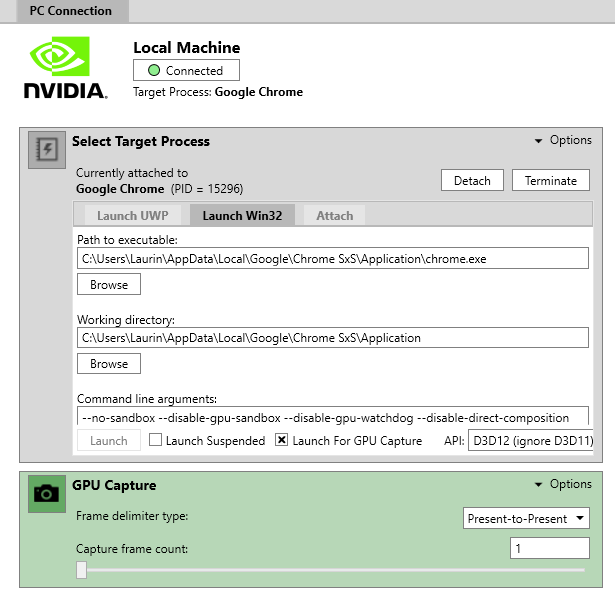
\includegraphics[width=\textwidth]{images/pix_options.png}
    \caption{Übersicht der Optionen zum Starten von \textit{Google Chrome Canary} in \textit{Microsoft PIX on Windows} \cite{microsoft:pix}. Bildschirmaufnahme durch Verfasser.}
    \label{fig:pix_options}
\end{figure}

\begin{figure}
    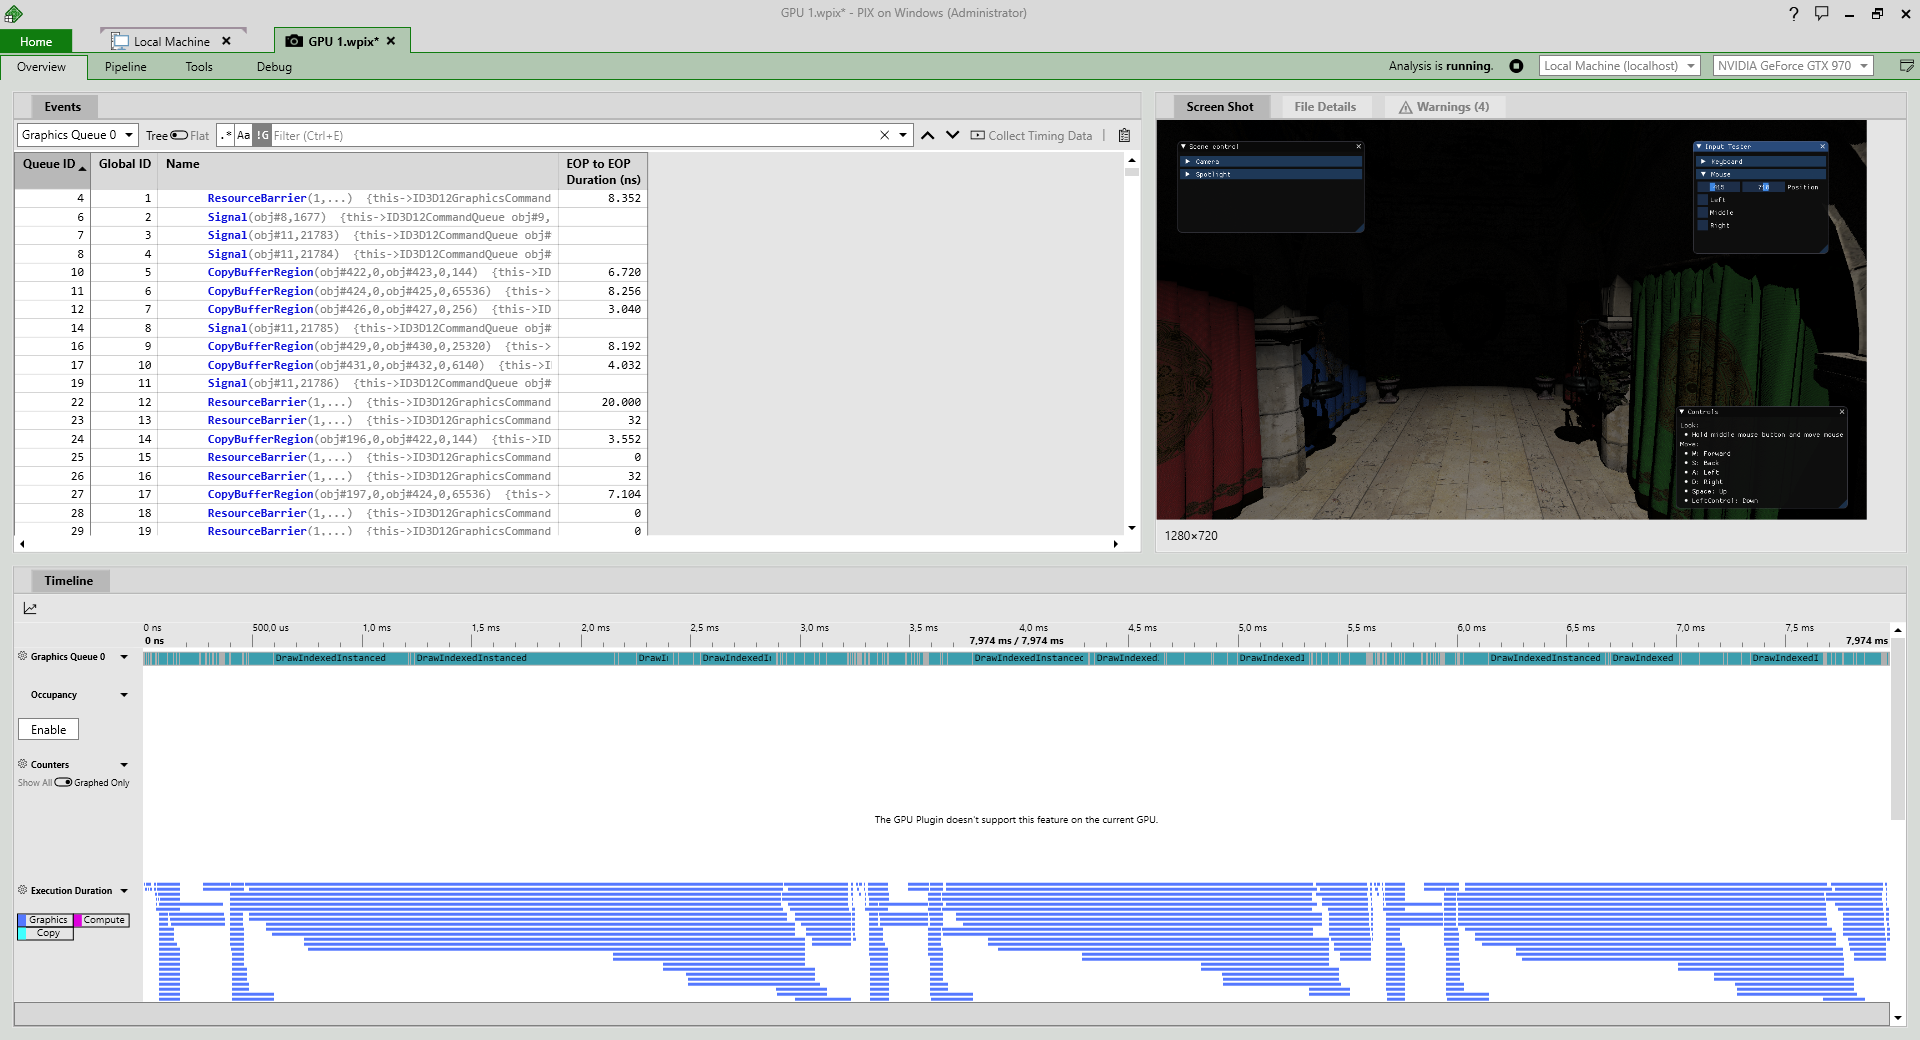
\includegraphics[width=\textwidth]{images/pix_overview.png}
    \caption{Anzeige nach der Erfassung eines Einzelbildes in \textit{Microsoft PIX on Windows} \cite{microsoft:pix}. Bildschirmaufnahme durch Verfasser.}
    \label{fig:pix_overview}
\end{figure}


%---
\chapter{Evaluierung}
\label{cha:evaluation}


%---
\chapter{Zusammenfassung und Ausblick}
\label{cha:zusammenfassung}

\section{Erreichte Ergebnisse}
\label{sec:ergebnisse}


\section{Ausblick}
\label{sec:ausblick}

\subsection{Erweiterbarkeit der Ergebnisse}
\label{sub:erweiterbarkeit}

\subsection{Übertragbarkeit der Ergebnisse}
\label{sub:uebertragbarkeit}


%-----------------------------------------------------------------------
\addcontentsline{toc}{chapter}{Referenzen}
\printbibliography[title={Referenzen}]

\appendix

%---
\chapter{Anhang A}
\label{appendix:a}
Dies ist der Quellcode zu der in Abbildung \ref{fig:spider_example_sponza} gezeigten Beispielanwendung. Die Anwendung lädt dabei das relativ komplexe 3D-Modell \textbf{Sponza} \cite{sponza} aus einer glTF-Datei \cite{khronos:gltf}, lässt den/die Anwender*in sich mit Hilfe einer steuerbaren Kamera im Raum bewegen und durch das UserInterface verschiedene Parameter der Szene verändern.
\begin{lstlisting}[language=C, label={lst:full_example}, caption={Kompletter C99-Quellcode zur Erstellung einer interaktiven 3D-Szene mit der \textbf{spider}-Engine}]
#include "spider/spider.h"

static SPLightID spot_light_id;
static uint32_t last_mouse_pos_x = 0;
static uint32_t last_mouse_pos_y = 0;
static const uint32_t surface_width = 1280;
static const uint32_t surface_height = 720;
static vec3 cam_rot = {0.0f, 0.0f, 0.0f};
static vec4 forward = {0.0f, 0.0f, 1.0f, 0.0f};
static float sensitivity = 2.0f;
static float vertical_limit = 0.01f;

void init(void) {
    // Lights have to be created before materials right now 
    const vec3 light_pos = {0.0f, 5.0f, 0.5f};
    const vec3 light_look_at = {2.0f, 0.0f, 0.0f};
    vec3 light_direction = {-1.0, -1.0f, 0.2f};
    // (float*) cast to prevent compiler warning 'incompatible-pointer-types-discards-qualifiers'
    // cglm takes no const pointers as arguments, even if it doesn't mutate the vectors
    glm_vec3_sub((float*)light_look_at, (float*)light_pos, light_direction);
    glm_vec3_normalize(light_direction);

    spot_light_id = spCreateSpotLight(&(SPSpotLightDesc){
            .pos = {light_pos[0], light_pos[1], light_pos[2]},
            .range = 40.0f,
            .color = {.r = 255, .g = 255, .b = 255},
            .dir = {light_direction[0], light_direction[1], light_direction[2]},
            .fov = glm_rad(70.0f),
            .power = 20.0f,
            .shadow_casting = &(SPLightShadowCastDesc){
                .shadow_map_size = 2048,
            },
        }
    );
    SP_ASSERT(spot_light_id.id != SP_INVALID_ID);

    /*SPSceneNodeID sponza_node_id = */spLoadGltf("assets/gltf/Sponza/Sponza.gltf");
}

bool update(float delta_time_s) {
    static bool show_controls = true;
    igBegin("Controls", &show_controls, ImGuiWindowFlags_None);
        igText("Look:");
            igBulletText("Hold right mouse button and move mouse");
        igText("Move:");
            igBulletText("W: Forward");
            igBulletText("S: Back");
            igBulletText("A: Left");
            igBulletText("D: Right");
            igBulletText("Space: Up");
            igBulletText("LeftControl: Down");
    igEnd();

    static bool scene_control = true;
    igBegin("Scene control", &scene_control, ImGuiWindowFlags_None);
    
    SPCamera* cam = spGetActiveCamera();
    glm_vec4_normalize(forward);

    if(cam) {
        if(spGetMouseButtonPressed(SPMouseButton_Right)) {
            vec2 relative_delta = {
                ((float)spGetMousePositionX() - (float)last_mouse_pos_x) / (float) surface_width,
                ((float)spGetMousePositionY() - (float)last_mouse_pos_y) / (float) surface_height
            };
            float rotation_speed = sensitivity * M_PI;
            cam_rot[1] -= rotation_speed * relative_delta[0]; // horizontal
            cam_rot[0] += rotation_speed * relative_delta[1]; // vertical
            cam_rot[0] = glm_clamp(cam_rot[0], (-M_PI * 0.5f) + vertical_limit, (M_PI * 0.5f) - vertical_limit);
        }
        memcpy(forward, (vec4){0.0f, 0.0f, 1.0f, 0.0f}, sizeof(vec4));
        mat4 rot = GLM_MAT4_IDENTITY_INIT;
        glm_euler_zyx(cam_rot, rot);
        glm_mat4_mulv(rot, forward, forward);

        cam->dir[0] = forward[0];
        cam->dir[1] = forward[1];
        cam->dir[2] = forward[2];
        vec3 sideward = {
            -forward[2],
            0.0f,
            forward[0],
        };
        glm_vec3_normalize(sideward);
        const float walk_speed = 2.0f;
        const float forward_movement = walk_speed * delta_time_s * (-1.0f * spGetKeyPressed(SPKey_S) + spGetKeyPressed(SPKey_W));
        const float sideward_movement = walk_speed * delta_time_s * (-1.0f * spGetKeyPressed(SPKey_A) + spGetKeyPressed(SPKey_D));
        const float upward_movement = walk_speed * delta_time_s * (-1.0f * spGetKeyPressed(SPKey_ControlLeft) + spGetKeyPressed(SPKey_Space));
        cam->pos[0] += forward[0] * forward_movement + sideward[0] * sideward_movement;
        cam->pos[1] += forward[1] * forward_movement + upward_movement;
        cam->pos[2] += forward[2] * forward_movement + sideward[2] * sideward_movement;
        
        if(igCollapsingHeaderTreeNodeFlags("Camera", ImGuiTreeNodeFlags_None)) {
            igSliderFloat("Look sensitivity##cam", &sensitivity, 0.0f, 5.0f, "%.1f", 1.0f);
            igSliderFloat("Vertical look limit##cam", &vertical_limit, 0.0f, M_PI * 0.5f, "%.2f", 1.0f);
            igSliderFloat3("Position##cam", (float*)&cam->pos, -10.0f, 10.0f, "%.2f", 1.0f);
            igSliderFloat3("Rotation (Rad)##cam", (float*)&cam_rot, -M_PI, M_PI, "%.2f", 1.0f);
            igSliderFloat("Vertical field of view (Rad)##cam", &cam->fovy, 0.01f, M_PI, "%.2f", 1.0f);
        }
    }

    last_mouse_pos_x = spGetMousePositionX();
    last_mouse_pos_y = spGetMousePositionY();
    
    SPLight* spot_light = spGetLight(spot_light_id);
    if(spot_light) {
        if(igCollapsingHeaderTreeNodeFlags("Spotlight", ImGuiTreeNodeFlags_None)) {
            igSliderFloat3("Position##light", (float*)&spot_light->pos, -50.0f, 50.0f, "%.1f", 1.0f);
            igSliderFloat("Field of view##light", &spot_light->fov, 0.0f, M_PI, "%.2f", 1.0f);
            igSliderFloat("Power##light", &spot_light->power, 0.0f, 1000.0f, "%.0f", 1.0f);
            igSliderFloat("Range##light", &spot_light->range, 0.0f, 1000.0f, "%.0f", 1.0f);
        }
    }
    igEnd();

    // return false if you want to quit
    return true;
}

int main() {
    spInit(&(SPInitDesc){
        .surface_size = {
            .width = surface_width,
            .height = surface_height
        },
        .update_func = update,
        .camera = {
            .pos = {0.0f, 2.0f, 0.0f},
            .dir = {0.0f, 0.0f, 1.0f},
            .look_at = {0.0f, 0.0f, 0.0f},
            .mode = SPCameraMode_Direction,
            .fovy = glm_rad(60.0f),
            .aspect = (float)surface_width / (float) surface_height,
            .near = 0.1f,
        },
        .pools.capacities = {
            .meshes = 128,
            .materials = 64,
            .render_meshes = 256,
            .lights = 1,
            .scene_nodes = 1024,
        },
        .show_stats = true,
    });

    init();

    spStart();
    return 0;
}
\end{lstlisting}

%---
%\chapter{Anhang B}


\end{document}